%% Main presentation %%
%%%%%%%%%%%%%%%%%%%%%%%%%%%%%%%%
%%%%%%%%%%%%%%%%%%%%%%%%%%%%%%%%

%% Title slide content %%
%% Template modfied by Kirsten Wright kirsten.wright@uwaterloo.ca 2024-01-14    %%
%% Based on template by Chris Carmona: carmona@stats.ox.ac.uk ; chriscarmona.me %%

\documentclass[notes=show]{beamer} %[notes=show/only]
\usepackage{tikz}

\newcommand\Wider[2][3em]{
% Has 2 parameters, addition to textwidth and content
\makebox[\linewidth][c]{%
  \begin{minipage}{\dimexpr\textwidth+#1\relax}
  \raggedright#2
  \end{minipage}%
  }%
}
% %% Packages %%
% %%%%%%%%%%%%%%%%%%%%%%%%%%%%%%%%
% %%%%%%%%%%%%%%%%%%%%%%%%%%%%%%%%

% \usepackage{tikz}
% \usepackage[UKenglish]{babel}
% \usepackage[utf8]{inputenc} % so we can input characters with accents (e.g. ő)

% \usepackage{statsbeamer}

% \usepackage{graphicx} % ease graphics management
% % \graphicspath{{images/}} % define folder with images
% % \graphicspath{{fig/}} % define folder with images
% \usefonttheme{serif} % change font to allow \textbf{}
% \usepackage{charter} % Nicer fonts

% \usepackage{amsmath,amsthm,amssymb} % for math equations

% % \usepackage{natbib} % richer citation
% \usepackage{breakcites} % avoid overfull hbox for long cites


%% Information (author, title, etc.) %%
% \setbeamerfont{title}{size*={2pt}}
\title{ Financialization of the Housing Market: A Contribution to Modern Urban Rent Theory}
% \author{Kirsten Wright} %\underline{Alyssa P. Hacker} \inst{1} \and Ben Bitdiddle \inst{2} \and Lem E. Tweakit \inst{2}}
\author{
  Author: Kirsten Wright \\
  Supervisors: Jangho Yang, Sean Geobey
}
% \institute{PhD Thesis Defensae}
\institute{PhD Thesis Defense \\[1ex] University of Waterloo}
%\date{February 10, 2024}
% \title[Short Title]{% short title for footer
%     Long and Descriptive Title
%     \vspace{0.5cm}
% }
% \author{ Your Name \and Your Collaborator}
% \institute{
%         \textit{Department of Statistics}\\
%         \textit{University of Waterloo}
%         \vspace{0.5cm}
% }
% \date[Venue and Date]{% short date for footer
%     Venue, Date
% }
\begin{document}


%% Slide content %%
%%%%%%%%%%%%%%%%%%%%%%%%%%%%%%%%
%%%%%%%%%%%%%%%%%%%%%%%%%%%%%%%%

% Title slide %
% %----------------------------%
{
    \setbeamertemplate{footline}{}
    \setbeamertemplate{headline}{}
    \setbeamercolor{background canvas}{bg=white}
    \maketitle   
}

% Field spheres image %
% %----------------------------%
\begin{frame}
\begin{figure}[!ht]
\centering
\resizebox{0.85\textwidth}{!}{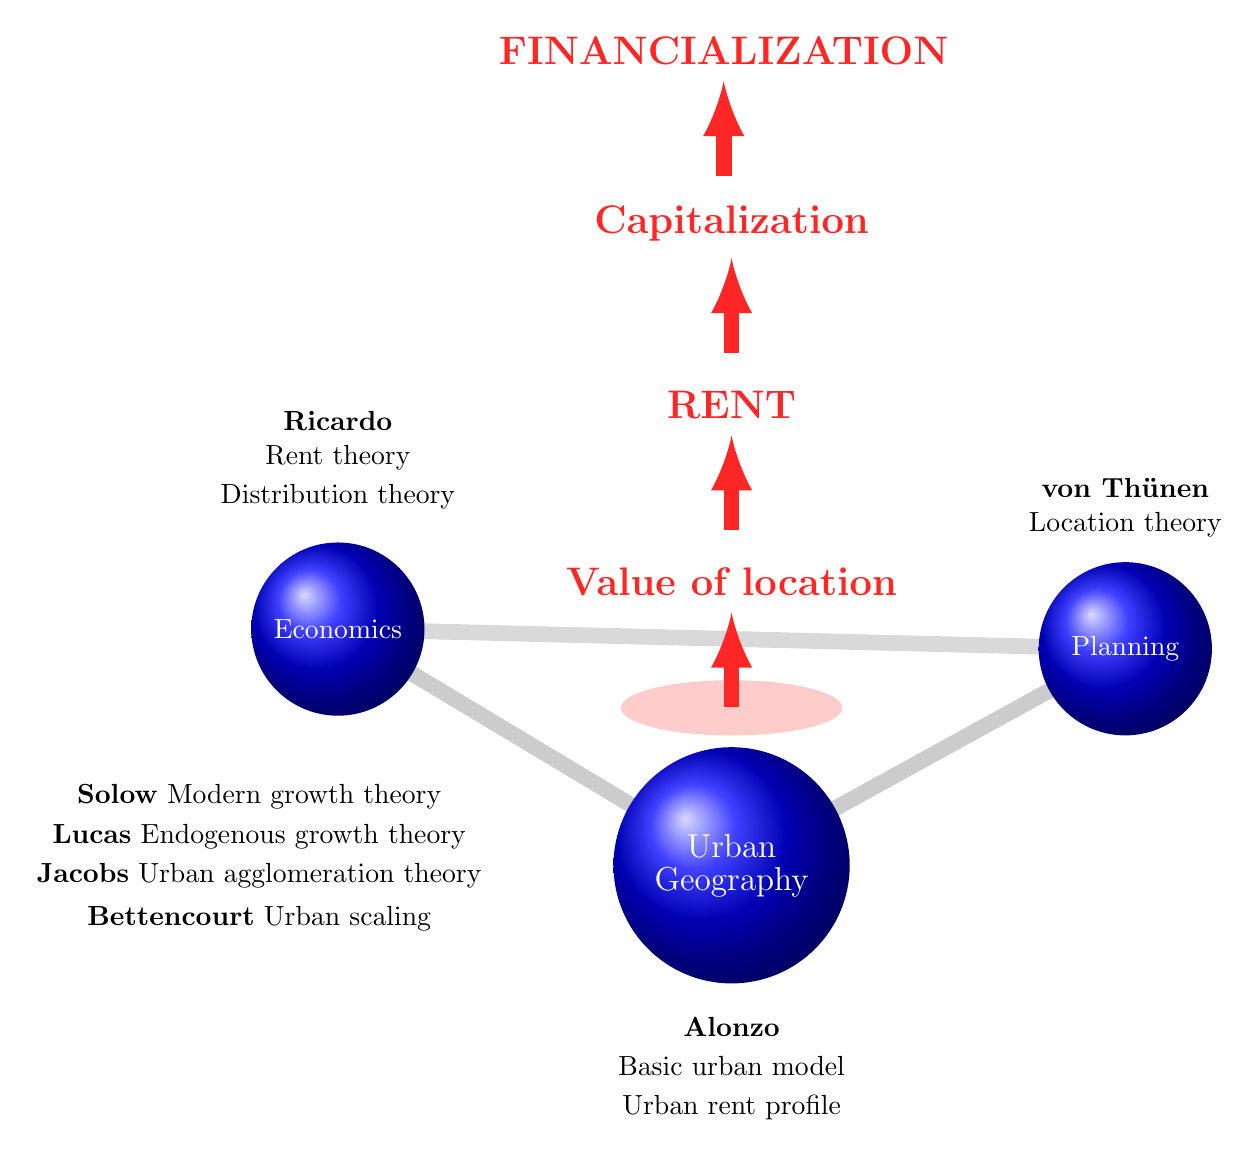
\begin{tikzpicture}{scale=.5}
% Find color for ball. Stop line short of node
\coordinate (planning) at (5,.75); % Preface
\coordinate (economics) at (-5,1); 
\coordinate (Ricardo) at (-5,1.4);
\coordinate (Solow) at (-6,1.25);
\coordinate (geography) at (0,-2); % History
\coordinate (finance) at (0,5); 

\draw [line width=2mm, black!15, ] (planning)--(economics);
\draw [line width=2mm, black!20, ] (geography)--(economics);
\draw [line width=2mm, black!20, ] (geography)--(planning);
%\draw [line width=2mm, black!25, ] (geography)--(finance);
%\draw [line width=2mm, black!20, ] (planning)--(finance);
%\draw [line width=2mm, black!20, ] (finance)--(economics);
%color=black!60!red
%\shade [ball color=blue!70] (5,5) circle (1.1cm)node[white] {\textbf{Planning}};
 
\node [circle,shading=ball,  minimum width=2.2cm, white, align=center] (ball) at (planning) {Planning};
\node [circle, shading=ball, minimum width=2.2cm, white, align=center] (ball) at (economics) {Economics};
\node [circle,shading=ball, minimum width=3cm, white, align=center] (ball) at (geography)[text width=2cm] {\large Urban \\ Geography};
%\node [circle, shading=ball, minimum width=2.4cm, white, align=center] (ball) at (finance)[text width=2cm] {Finance};
%\node at (-.3,-.1) [red] {\Large \textbf{RENT}};

\node at (planning) [above=1.8cm] {\textbf{von Th\"unen}};
\node at (planning) [above=1.3cm] {Location theory};

\node at (Ricardo) [above=2cm,]   {\textbf{Ricardo}};
\node at (Ricardo) [above=1.5cm] {Rent theory};
\node at (Ricardo) [above=1.0cm] {Distribution theory};

% \node at (Solow) [below=1.6cm, align=left] {\textbf{Solow:}};
\node at (Solow) [below=2.1cm, align=left] {\textbf{Solow} Modern growth theory};
\node at (Solow) [below=2.6cm, align=left] {\textbf{Lucas} Endogenous growth theory};
\node at (Solow) [below=3.1cm, align=left] {\textbf{Jacobs} Urban agglomeration theory};
\node at (Solow) [below=3.65cm, align=left] {\textbf{Bettencourt} Urban scaling};

\node at (geography) [below=1.8cm] {\textbf{Alonzo}};
\node at (geography) [below=2.3cm] {Basic urban model};
\node at (geography) [below=2.8cm] {Urban rent profile};
%\node [circle, shading=ball, minimum width=2.4cm, white, align=center] (ball) at (finance)[text width=2cm] {Finance};

\fill[red!20] (0,0) ellipse (40pt and 10pt);
%\node[red]at (1.2,0) {\large SPACE};
\begin{scope}[shift={(0,-.34)}]
\draw [line width=2mm, red!85, -latex ] (-.1, 7.1)--++(0,1.2)node[above=-.1] {\Large \textbf{FINANCIALIZATION}};
\draw [line width=2mm, red!85, -latex ] (0, 4.85)--++(0,1.2)node[above=-.1] {\Large \textbf{Capitalization}};
\draw [line width=2mm, red!85, -latex ] (0, 2.6)--++(0,1.2)node[above=-.1] {\Large \textbf{RENT}};
\draw [line width=2mm, red!85, -latex ] (0, .35)--++(0,1.2)node[above] {\Large \textbf{Value of location}};
%\draw [line width=2mm, red!85, -latex ] (0, -2)--++(0,-.8)node[above=-.1]  {\Large \textbf{SPACE}};
\end{scope}
\end{tikzpicture}


% % JUST THE BOTTOM 3 BALLS FOR PLANNING, ECONOMICS AND URBAN GEOGRAPHY
% \begin{figure}
% \begin{tikzpicture}{scale=.5}
% % find color cotrol for ball. Tind way to stop line short of node
% \coordinate (planning) at (-5,1);%PREFACE
% \coordinate (economics) at (5,.75);%
%  \coordinate (geography) at (-.5,-2); %history
% \coordinate (finance) at (0,5); %

% \draw [line width=2mm, black!15, ] (planning)--(economics);
% \draw [line width=2mm, black!20, ] (geography)--(economics);
% \draw [line width=2mm, black!20, ] (geography)--(planning);

% %\draw [line width=2mm, black!25, ] (geography)--(finance);
% %\draw [line width=2mm, black!20, ] (planning)--(finance);
% %\draw [line width=2mm, black!20, ] (finance)--(economics);
% \node [circle,shading=ball, minimum width=2.1   cm, white, align=center] (ball) at (planning) {Planning};
% \node [circle,shading=ball, minimum width=2.2cm, white, align=center] (ball) at (economics) {Economics};
% \node [circle,shading=ball, minimum width=3cm, white, align=center] (ball) at (geography)[text width=2cm] {\large Urban\\ Geography};
% %\node [circle, shading=ball, minimum width=2.4cm, white, align=center] (ball) at (finance)[text width=2cm] {Finance};

% \node at (-.3,-.1) [red] {\Large \textbf{Space}};
% \end{tikzpicture}
% \caption{The common concern of three fields topic }
%     \label{fig-three-fields}
% \end{figure}}
% 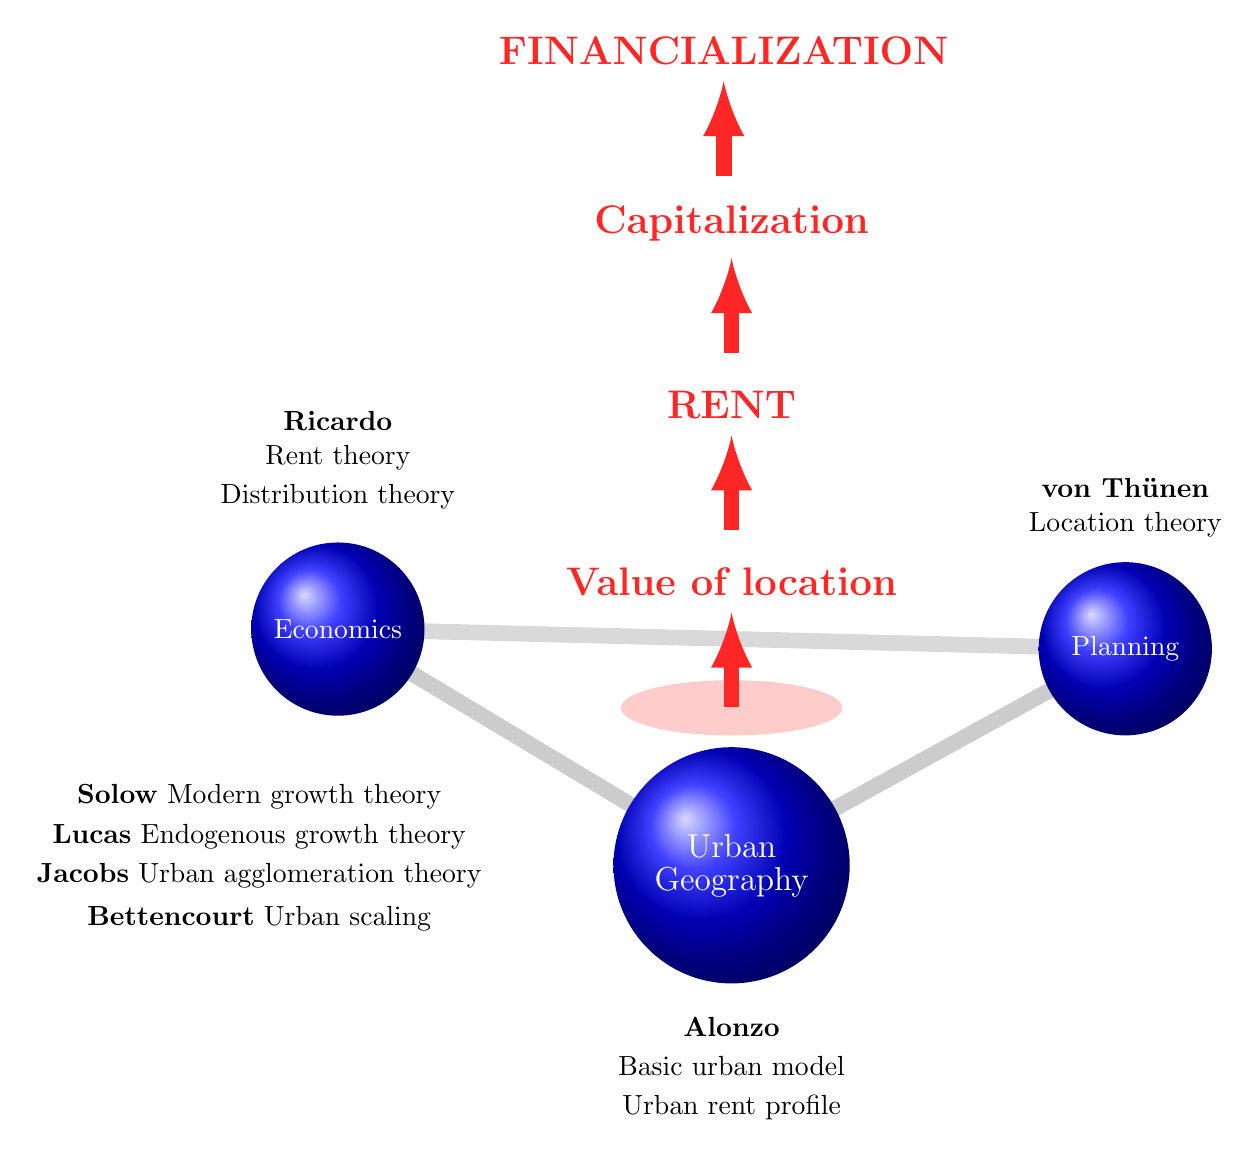
\begin{tikzpicture}{scale=.5}
% Find color for ball. Stop line short of node
\coordinate (planning) at (5,.75); % Preface
\coordinate (economics) at (-5,1); 
\coordinate (Ricardo) at (-5,1.4);
\coordinate (Solow) at (-6,1.25);
\coordinate (geography) at (0,-2); % History
\coordinate (finance) at (0,5); 

\draw [line width=2mm, black!15, ] (planning)--(economics);
\draw [line width=2mm, black!20, ] (geography)--(economics);
\draw [line width=2mm, black!20, ] (geography)--(planning);
%\draw [line width=2mm, black!25, ] (geography)--(finance);
%\draw [line width=2mm, black!20, ] (planning)--(finance);
%\draw [line width=2mm, black!20, ] (finance)--(economics);
%color=black!60!red
%\shade [ball color=blue!70] (5,5) circle (1.1cm)node[white] {\textbf{Planning}};
 
\node [circle,shading=ball,  minimum width=2.2cm, white, align=center] (ball) at (planning) {Planning};
\node [circle, shading=ball, minimum width=2.2cm, white, align=center] (ball) at (economics) {Economics};
\node [circle,shading=ball, minimum width=3cm, white, align=center] (ball) at (geography)[text width=2cm] {\large Urban \\ Geography};
%\node [circle, shading=ball, minimum width=2.4cm, white, align=center] (ball) at (finance)[text width=2cm] {Finance};
%\node at (-.3,-.1) [red] {\Large \textbf{RENT}};

\node at (planning) [above=1.8cm] {\textbf{von Th\"unen}};
\node at (planning) [above=1.3cm] {Location theory};

\node at (Ricardo) [above=2cm,]   {\textbf{Ricardo}};
\node at (Ricardo) [above=1.5cm] {Rent theory};
\node at (Ricardo) [above=1.0cm] {Distribution theory};

% \node at (Solow) [below=1.6cm, align=left] {\textbf{Solow:}};
\node at (Solow) [below=2.1cm, align=left] {\textbf{Solow} Modern growth theory};
\node at (Solow) [below=2.6cm, align=left] {\textbf{Lucas} Endogenous growth theory};
\node at (Solow) [below=3.1cm, align=left] {\textbf{Jacobs} Urban agglomeration theory};
\node at (Solow) [below=3.65cm, align=left] {\textbf{Bettencourt} Urban scaling};

\node at (geography) [below=1.8cm] {\textbf{Alonzo}};
\node at (geography) [below=2.3cm] {Basic urban model};
\node at (geography) [below=2.8cm] {Urban rent profile};
%\node [circle, shading=ball, minimum width=2.4cm, white, align=center] (ball) at (finance)[text width=2cm] {Finance};

\fill[red!20] (0,0) ellipse (40pt and 10pt);
%\node[red]at (1.2,0) {\large SPACE};
\begin{scope}[shift={(0,-.34)}]
\draw [line width=2mm, red!85, -latex ] (-.1, 7.1)--++(0,1.2)node[above=-.1] {\Large \textbf{FINANCIALIZATION}};
\draw [line width=2mm, red!85, -latex ] (0, 4.85)--++(0,1.2)node[above=-.1] {\Large \textbf{Capitalization}};
\draw [line width=2mm, red!85, -latex ] (0, 2.6)--++(0,1.2)node[above=-.1] {\Large \textbf{RENT}};
\draw [line width=2mm, red!85, -latex ] (0, .35)--++(0,1.2)node[above] {\Large \textbf{Value of location}};
%\draw [line width=2mm, red!85, -latex ] (0, -2)--++(0,-.8)node[above=-.1]  {\Large \textbf{SPACE}};
\end{scope}
\end{tikzpicture}


% % JUST THE BOTTOM 3 BALLS FOR PLANNING, ECONOMICS AND URBAN GEOGRAPHY
% \begin{figure}
% \begin{tikzpicture}{scale=.5}
% % find color cotrol for ball. Tind way to stop line short of node
% \coordinate (planning) at (-5,1);%PREFACE
% \coordinate (economics) at (5,.75);%
%  \coordinate (geography) at (-.5,-2); %history
% \coordinate (finance) at (0,5); %

% \draw [line width=2mm, black!15, ] (planning)--(economics);
% \draw [line width=2mm, black!20, ] (geography)--(economics);
% \draw [line width=2mm, black!20, ] (geography)--(planning);

% %\draw [line width=2mm, black!25, ] (geography)--(finance);
% %\draw [line width=2mm, black!20, ] (planning)--(finance);
% %\draw [line width=2mm, black!20, ] (finance)--(economics);
% \node [circle,shading=ball, minimum width=2.1   cm, white, align=center] (ball) at (planning) {Planning};
% \node [circle,shading=ball, minimum width=2.2cm, white, align=center] (ball) at (economics) {Economics};
% \node [circle,shading=ball, minimum width=3cm, white, align=center] (ball) at (geography)[text width=2cm] {\large Urban\\ Geography};
% %\node [circle, shading=ball, minimum width=2.4cm, white, align=center] (ball) at (finance)[text width=2cm] {Finance};

% \node at (-.3,-.1) [red] {\Large \textbf{Space}};
% \end{tikzpicture}
% \caption{The common concern of three fields topic }
%     \label{fig-three-fields}
% \end{figure}
% \includegraphics[width=0.6\textwidth]{fig/fields}
% \caption[Linking space and urban rents to the effects of financialization.]{Space and urban rents play a foundational role in urban economics, geography, and planning. We extend the analysis of urban rents to model the effects of financialization.}
\label{fig-fields}
\end{figure}
\end{frame}
\note[enumerate]{\item Three fields that are concerned with space and cities 

Three contributions from this thesis
\item I bring together models and theories from all three
\item I apply the theory of land to the urban distribution problem
\item I link productivity to locational rents (middle of figure)
\item I show financialization to capturing the locational rents and the productivity of the city
\item I begin exploring the feedback form financialization to productivity}



% %----------------------------%
\begin{frame}{Production and the city}
\huge 
$Y=AN^\beta$ {\normalsize \hfill \textbf{Scale literature and Jacobs}\\\hfill $N =$ population}
\vspace{.5cm}

$y=\:A\quad \;k^\alpha n^\beta$ {\normalsize \hfill \textbf{Neoclassical production function}\\ \hfill$n =$ firm workforce}
\vspace{.5cm}

$y=\:AN^\gamma k^\alpha n^\beta$ {\normalsize \hfill \textbf{Synthesis in our model}\\\hfill $N = f*n, \qquad f=$ number of firms}



\end{frame}
\note[enumerate]{\item the first is a fact.
\item the second in a an attempt to provide a theory.  $\alpha +\beta\le 1$ It is clearly incomplete empirically
\item the third is my model, which is a synthesis drawing on modern growth theory. 
\item We can show that heuristically city grows if  $\gamma>0$. Say the firm size is a constant.  Then $N=zF$ and $Y=Fy$ 
$Y\propto FAz^\gamma F^\gamma *c\propto c'F^{1+\gamma}  $ 

(Then  $\beta$ in the first equation is $1+\gamma$)

}
% %----------------------------%
\begin{frame}{Increasing returns in the city}

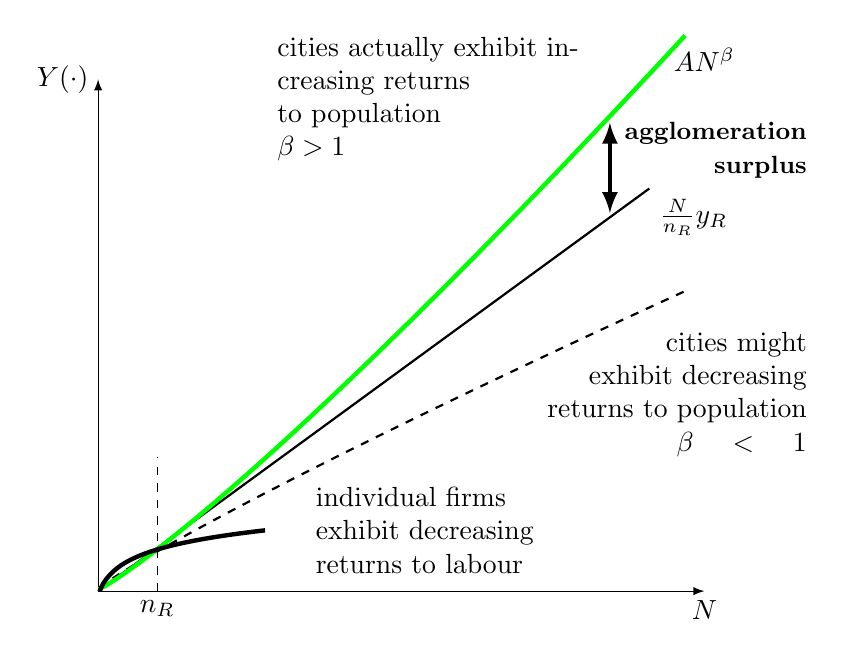
\begin{tikzpicture}[scale=.5, my plot/.style={thick, smooth, samples=100, domain=0.1:2.2},
plot2/.style={thick, smooth, samples=100, domain=0.1:14.99},
                    my grid/.style={dashed,opacity=0.5, every node/.style={black,opacity=1}},
                    my axis/.style={latex-latex}]
 
 \draw[my axis] (0,13)node[left] {$Y(\cdot)$} --(0,0)-- (15.4, 0) node[below] {$N$}; %creates the axis a little 

\coordinate (origin) at (0,0);
\def\x{0.45}
\def\y{2.1}
\def\b {$15/(2*ln(\y)+.05)$};
%\def\p{0.55} % define the x, y and p )(midpointvalues
%\draw[my plot] (0,0) plot (\x,{ln(\x)});  %Draws curve
%\draw[my plot] (0,0) plot ({\x-.08},{2.3+ln(\x)}); 
\coordinate (Uy) at (\y,{2*ln(\y)+.05});

% THREE SCALE POSSIBILITIES
\draw [thick, ](0,0)--(14, 10.22583)node[below right]{$\frac{N}{n_R}y_R$};   %diagonal line CRS
\draw[plot2, dashed] (0,0) plot ({\x-.08},{(\x)^0.9/1.5 }); %DRS
\draw[plot2, ultra thick, green] (0,0) plot ({\x-.08},{(\x/1.5)^1.15});%
\node at (15.4, 13.5){$AN^\beta$};

%  TEXT
\node at (13.8,12.5) [left, text width=4.5cm]{ cities actually exhibit increasing returns\\ to population\\ $\beta>1$};%IRS
\node at (13.5,5)[text width=4.5cm, align=right] {cities might\\ exhibit decreasing \\returns to population \\ $\beta<1$};% DRS

% ARROW
\draw[latex-latex, ultra thick] (13, 11.9)--(13, 9.6);
\node at (15.5, 11.2)[ text width=2.5cm, align=right]{\small\textbf{agglomeration\\ surplus}};

\begin{scope}[ yscale=1,xscale=2]% shift={(1.9,0)} ,
	\coordinate (Uy) at (\y, {2.3+ln(\y)});
  \draw[my plot,ultra thick] (0,0) plot ({\x-.08},{1.15+ln(\x)/2})node[right=.5cm, text width=3.9cm]{individual firms\\ exhibit decreasing\\ returns to labour}; % production function for generic ferm
	\draw[dashed](.75, 0)node[below]{$n_R$} --(.75, 3.4);
\end{scope}
\end{tikzpicture}

\end{frame}
\note[enumerate]{\item the straight solid line is what you get if firms choose the optimal size and just replicate.
\item The green is the observed expansion path
\item It happens if every business has DRS but $\gamma>0$
}

% %----------------------------%
\begin{frame}{Population model}
\huge 
$w=\frac{\beta y} {n}$ {\normalsize \hfill \textbf{firm behavior}\\\hfill $ w =$ wage}
\vspace{.5cm}

$\omega=w-\psi$ {\normalsize \hfill \textbf{wage premium}\\\hfill $ \psi=$ subsistence wage}
\vspace{.5cm}

$N= \frac{(w-\psi)^2}{2c^2 }$ {\normalsize \hfill \textbf{population equilibrium}\\\hfill $ c=$ transportation cost}

\end{frame}
\note[itemize]{\Large
\item We need a wage-setting process. The first equation is just the marginal product of labour with the Cobb-Douglas
\item The second is my modelling decision about how to connect the production sector to the urban system in my model NEATLY.
\item the third calculates the equilibrium population in the Alonzo model 
\hspace{1cm}
We have connected the  circle
}

% %----------------------------%

% %----------------------------%
\begin{frame}{The production system feedback}\framesubtitle{The Alonzo-Jacobs Cycle}
% \begin{figure}[!ht]
\vspace{-.5cm}
\Wider[4em]{\centering
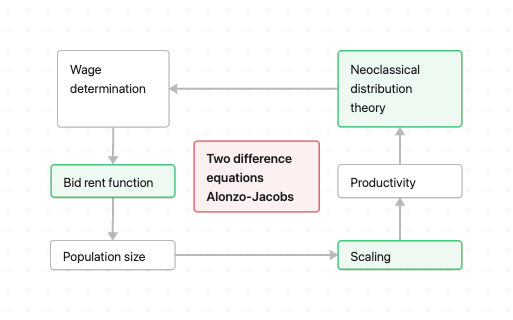
\includegraphics[scale=.75,trim={.5cm 0cm 0 1.cm},clip]{fig/flow-alonso-jacobs-cycle.png}
}
% \caption[Production system.]{The production system component, incorporating the urban scaling of wealth in the urban spatial model. We name this coupling of two difference equations the Alonso-Jacobs cycle.}
% \label{fig-alonso-jacobs-cycle}
% \end{figure}

\vspace{-1.5cm}
\hspace{1cm}ALONZO \hspace{5.5cm} JACOBS
\end{frame}


\note[itemize]{\large
\item A classic positive feedback cycle
\item Green refers to a theory and grey boxes to the calculations
\item We could represent the model with two difference equations, but this is an agent-based model.
\item most of the coding happens in the bidding (and housing allocation)
\item most of the theory is involved in what happens in the other boxes and trying to makes sure that those processes are economically plausible and that different theories - say about wage determination  - can be plugged in if I want to. 

}

% %----------------------------%
\begin{frame}{The housing market with three classes}
\begin{center}
 \vspace{-.5cm}   
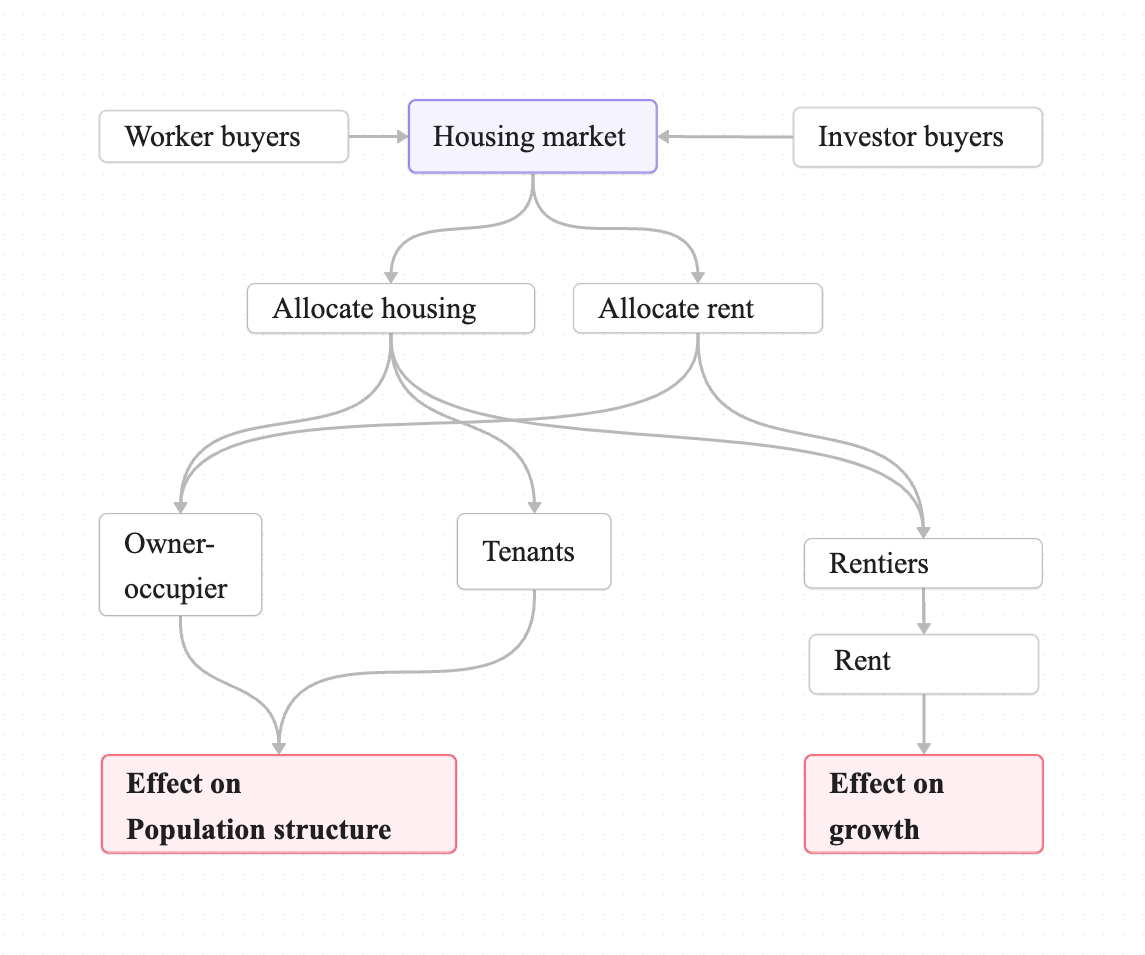
\includegraphics[scale=.14,trim={.5cm 1cm 0 1.5cm},clip]{fig/flow-impacts.png}
\end{center}

% \caption[The housing market component of the model.]{The housing market component. Financialization affects both the allocation of housing and its allocation of rents.}
\end{frame}
\note[itemize]{\Large
\item Now we are into the complicated part of the modelling
\item In the housing market investors and workers bid for existing housing. 
\item I have an equation that takes most of a chapter to explain to calculate how much each agent would bid for a property. 
\item Then I model each sale as a multi-bidder auction.

}
% %----------------------------%
\begin{frame}{The financialization component}
% \begin{figure}[!ht]
\centering
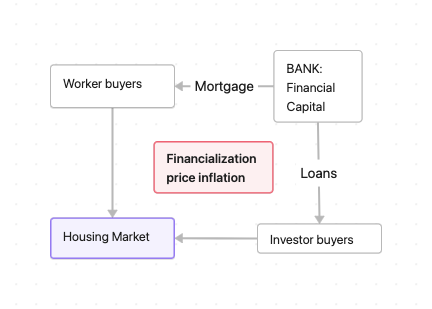
\includegraphics[scale=.75]{fig/flow-financialization.png}
% \caption[The financialization component of the model.]{The financialization component. There is a feedback loop in which new investors drive up demand and thus drive up prices.}
% \label{fig-financial-cycle}
% \end{figure}
\end{frame}
\note[itemize]{\Large
\item But I had to go back one more step to bring in the financial sector
\item Notice how finance -capital - enters both directly through investor purchases and less directly through mortgages:
\item "I don't own my house: the bank does!"
}


% %----------------------------%
\begin{frame}{12 experiments, 84 results}
\begin{enumerate}\Huge
    \item six policy variables
    \item two states of the world
    \item seven outcome variables for each 
\end{enumerate}
\end{frame}% %
\note[]{\Large
I'm only reporting 12 experiments on a single parametrization of the basic model. 

}


% %----------------------------%
\begin{frame}{Experiment: Capital gains tax on investors with no linkage}
\begin{tikzpicture} 
\node at (.7cm,10cm){
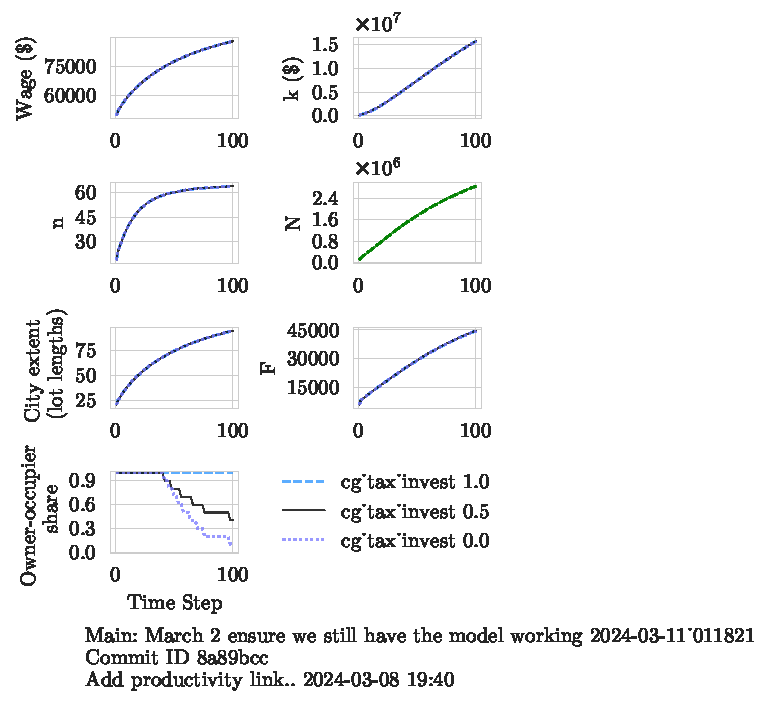
\includegraphics[scale=.8, trim={0 1.4cm 4cm 0},clip]{fig/cg_tax_invest-Main-011821.pdf}};
\pause

\node at (6cm,13.5){wage, capital stock};
\node at (6cm,11.56){workforce, population};
\node at (6.1cm,9.6){city radius, number of firms};
\node at (6cm,7.7){owner-occupier share};
\end{tikzpicture}
\end{frame}% %

\note[itemize]{\Large
\item 100-year evolution of an city economy 
\item Population grows to 2.4 million
\item Arbitrary firm technology  most growth falls on increasing the number of firms

\item A capital gains tax does not affect production 
\item It does affect the ownership ratio profoundly.
\item This is an important result for policy makers to know
}

% %----------------------------%
\begin{frame}{Experiment: Adding productivity impacts}
     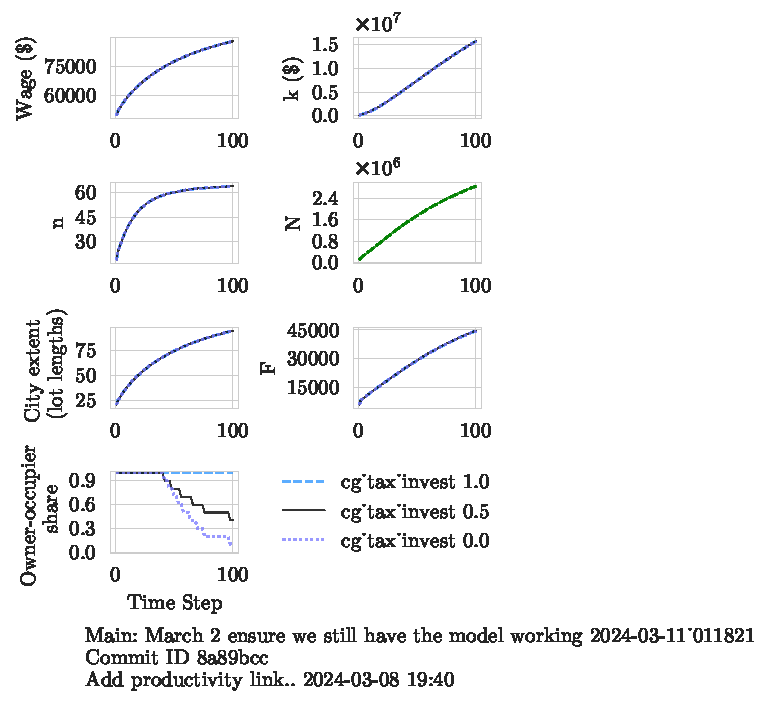
\includegraphics[scale=.55, trim={0 1.4cm 4.5cm 0},clip]{fig/cg_tax_invest-Main-011821.pdf} 
    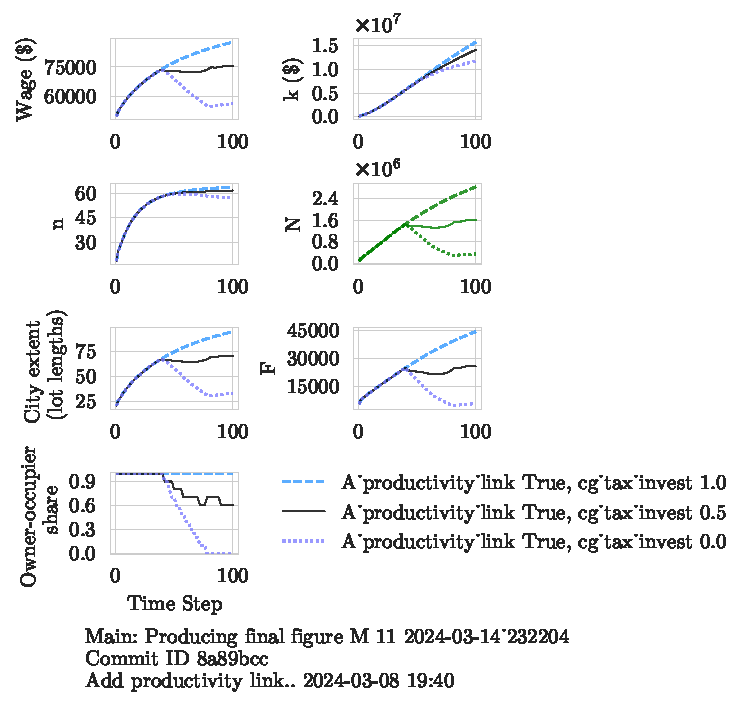
\includegraphics[scale=.55, trim={0 1.4cm 3.8cm 0},clip]{fig/With-productivity_linkcg_tax_invest-232204.pdf} 
\end{frame}% %
\note[itemize]{\large
\item comparing the same case with a strong linkage to productivity 
\item effect of capital gains tax on ownership is larger with linkage. \textbf{Linkage make this policy matter more.} 
\item \textbf{With linkage} a higher  CGT for investors is better for all production-side variables and increases city size
\item a 100\% capital gains tax does not affect production side or ownership
\item 50\%  does affect population considerably 
\item IF LOWER than the cgtax for owners-occupiers it leads to a population crash. 
\item These are important results for policy makers to know
}

\note[]{It is tempting to talk about why these specific results happen and what model parameter of behaviour assumptions might affect them. 

I expect to get into those discussions with policy makers

This is a modelling project - For mew the real question is, "Can we build a model consistent with theory that actually address the emerging challenges of our cities, and can we build on that helps us grapple with the relatively recent growth of finacialization. 

I hope that I have done that. 

Let's look at some more results.
}


% %----------------------------%
\begin{frame}{The model tells us that }
\begin{itemize}
 %\item In the absence of linkages between the housing market and the production sector, of the policy tools we consider, only density and transportation cost and capital gains taxation have much effect. 

 \only<1>{\color{red}}\item In the presence of linkages, policy tools have much more dramatic effects. This is potentially very important result. 
 \pause

 \only<2>{\color{red}}\item  a capital gains tax on speculative investment without linkage increases owner occupancy. 

 \only<2>{\color{red}}\item With a productivity linkage, a a capital gains tax on speculation increases wages and the size of the city. 
 \pause
  \only<3>{\color{red}}\item  A capital gains tax on owner-occupiers above the level of on investors has a powerfully negative effect on population and wages.
\end{itemize}
\end{frame}% %----------------------------%

\note{\huge \color{red} You can put in more experiments here if you think it would help.}

\setbeamercovered{transparent=20}

\begin{frame}{Summarizing other experiments}
\begin {itemize}[<alert@+>]\Large 


 \item  The cost of capital has surprisingly little effect on any variables in either case.

 \item  Transportation cost has a strong effect on wages and city size as expected 
 
  \item Low transportation costs with financial system spillovers appear to induce something like cyclical behaviour.

 \item  Increasing density increases the population but does not affect wages or city extent.
\end{itemize}
\end{frame}% %----------------------------%


\begin{frame}{Results} \Large
\begin {itemize}[<+-|alert@+>]
 \item A restrictive mortgage market does not affect the production sector or city size.

 \item  Increasing property taxes reduces owner occupiers, but has only a small effect on city size when there is no linkage. 
 
 \item  With linkage increasing property taxes depresses wages, population and city size.
\end{itemize}
\end{frame}% %----------------------------%



% %----------------------------%
\begin{frame}{Ex styles for presenting equations}
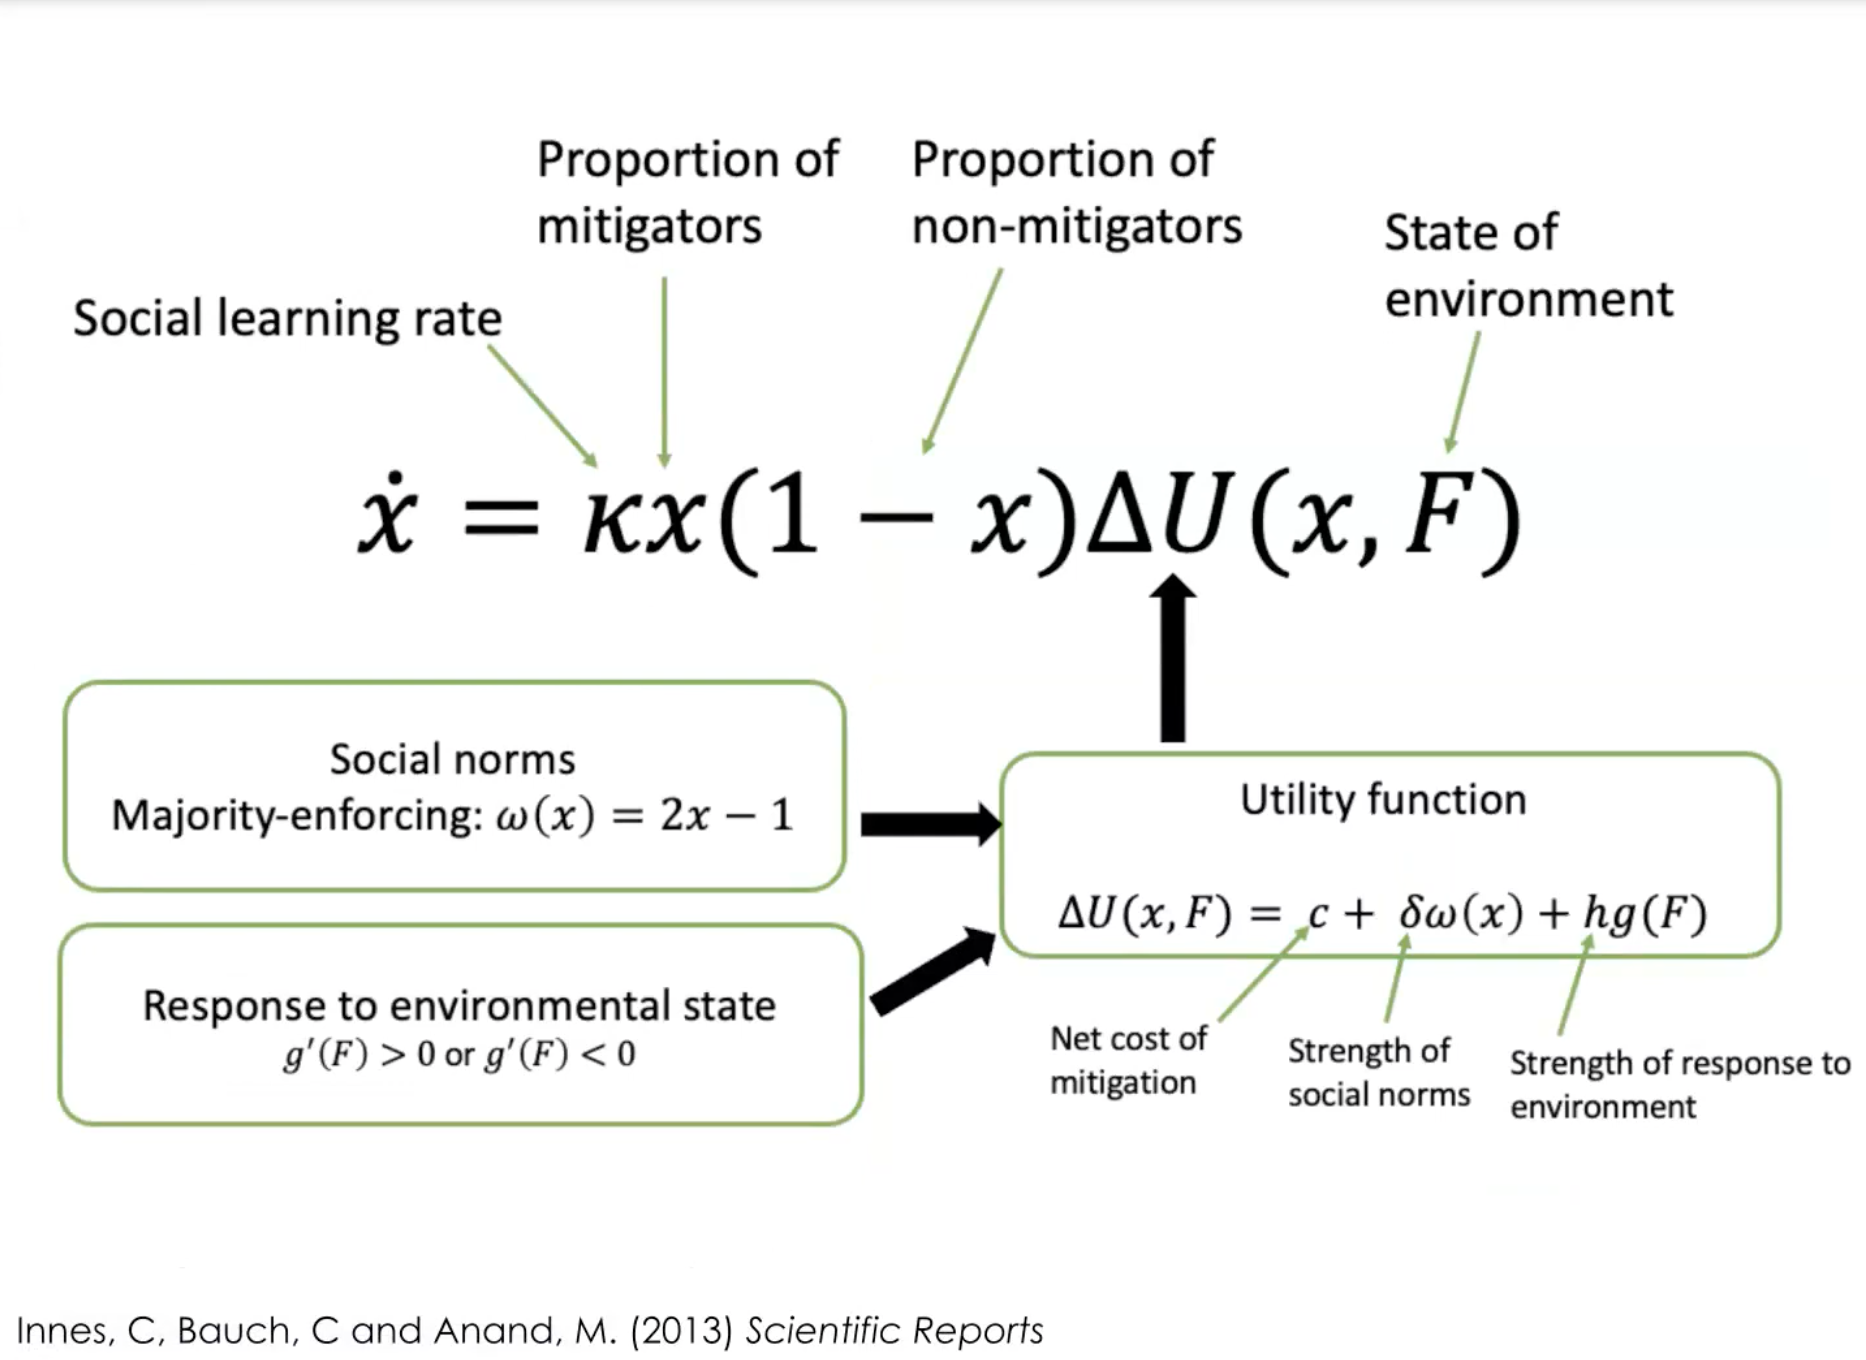
\includegraphics[scale=.35]{fig/example_figures/eqn-ex-1.png}
\end{frame}% %----------------------------%
\begin{frame}{Ex styles for presenting equations}
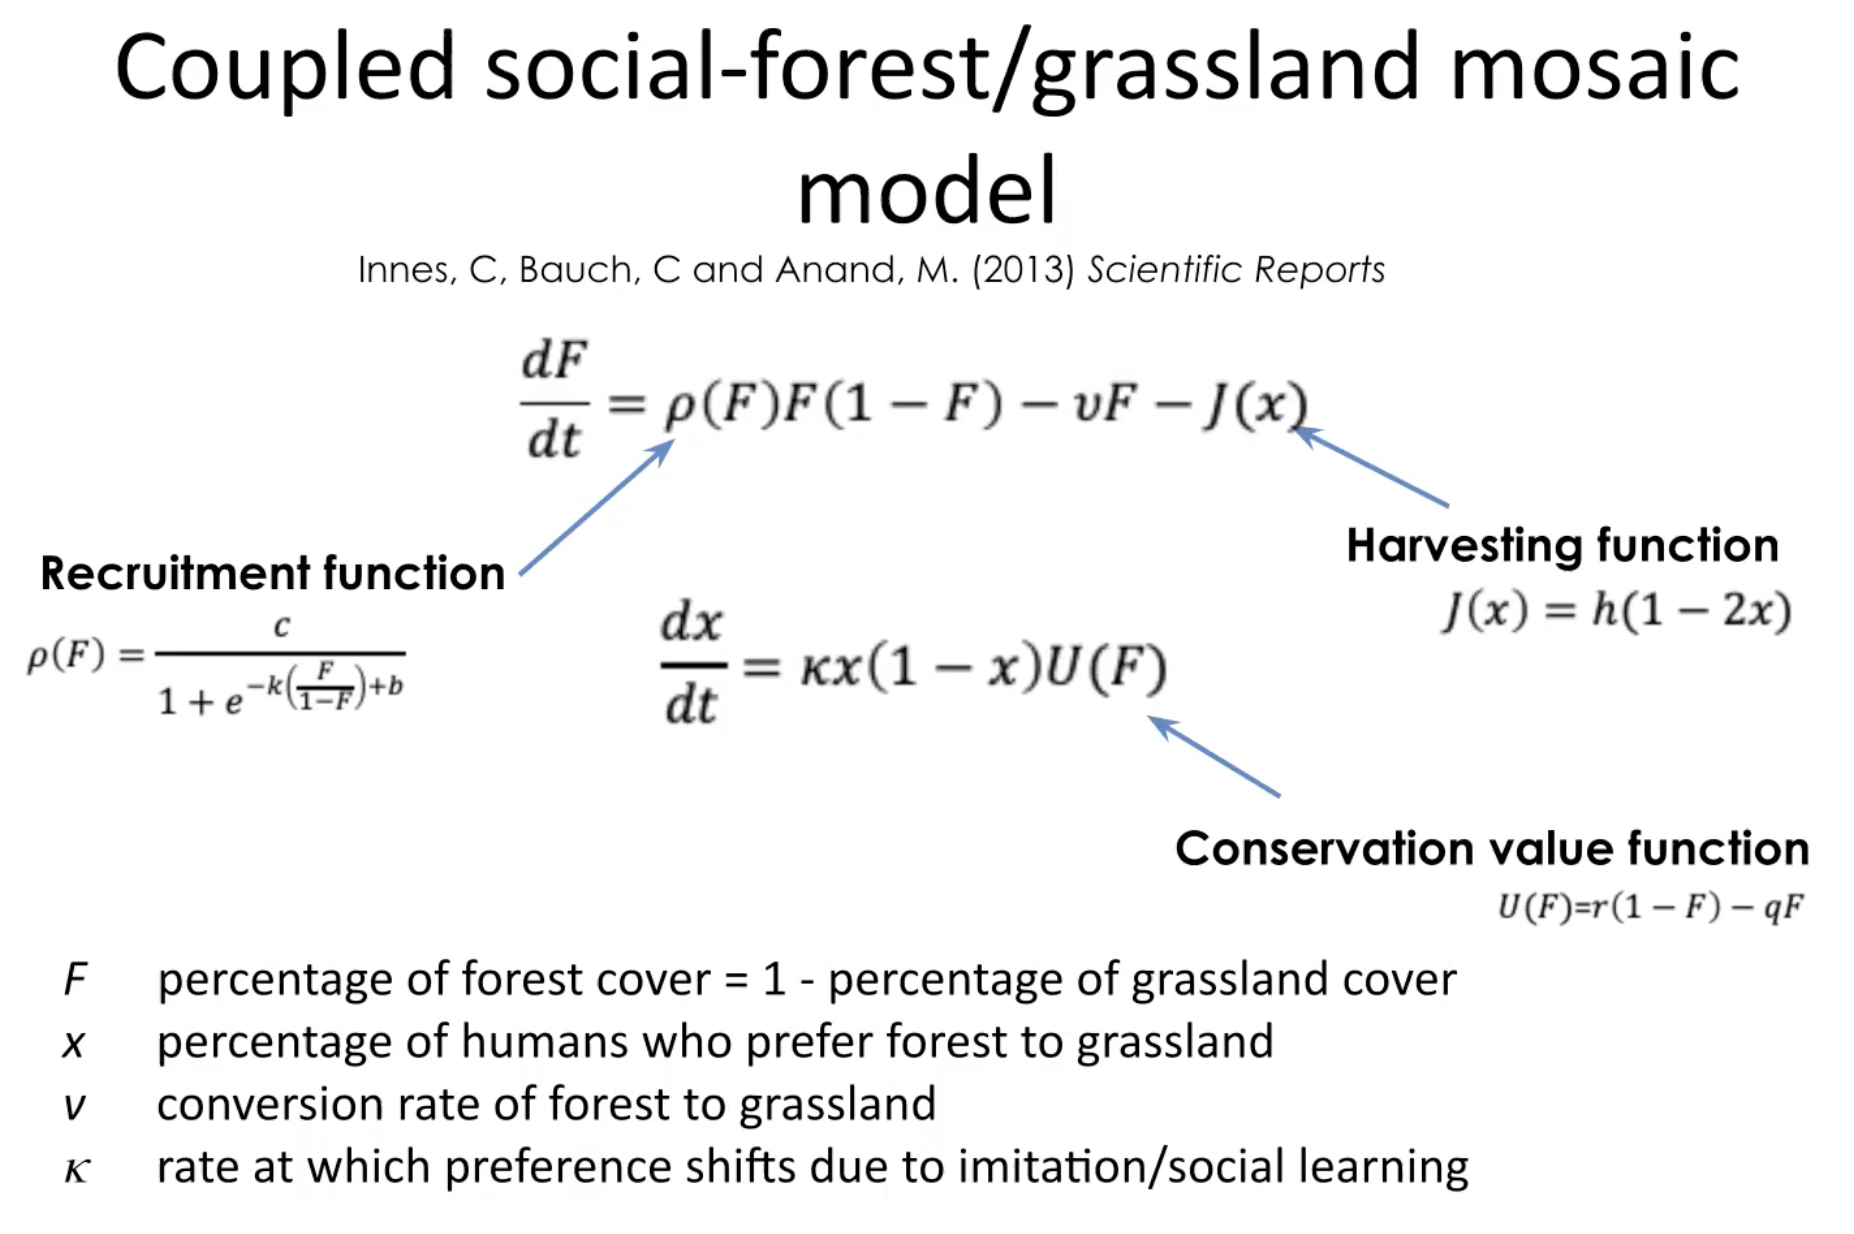
\includegraphics[scale=.35]{fig/example_figures/eqn-ex-2.png}
\end{frame}% %----------------------------%
\begin{frame}{Frame Title}
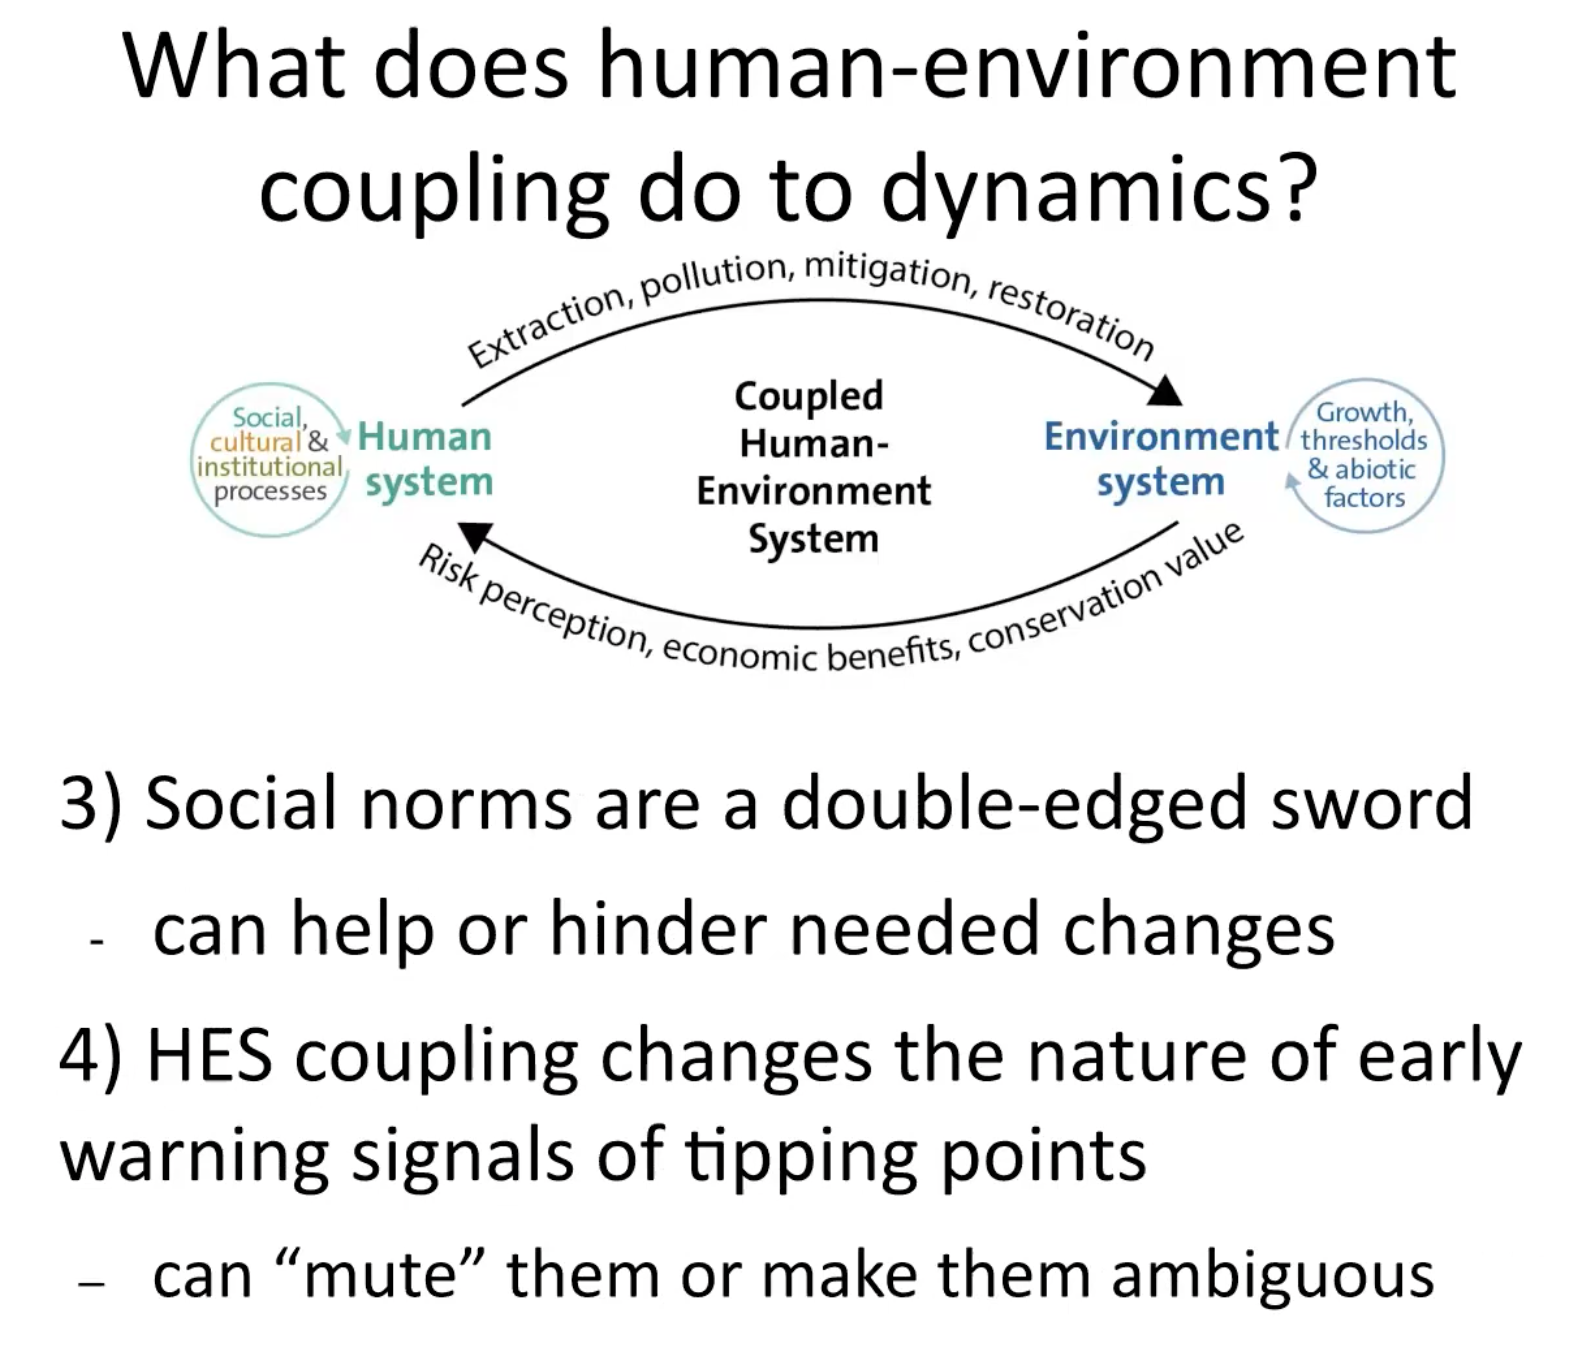
\includegraphics[scale=.35]{fig/example_figures/feedbk-eqn-1.png}
\end{frame}
\begin{frame}{Frame Title}
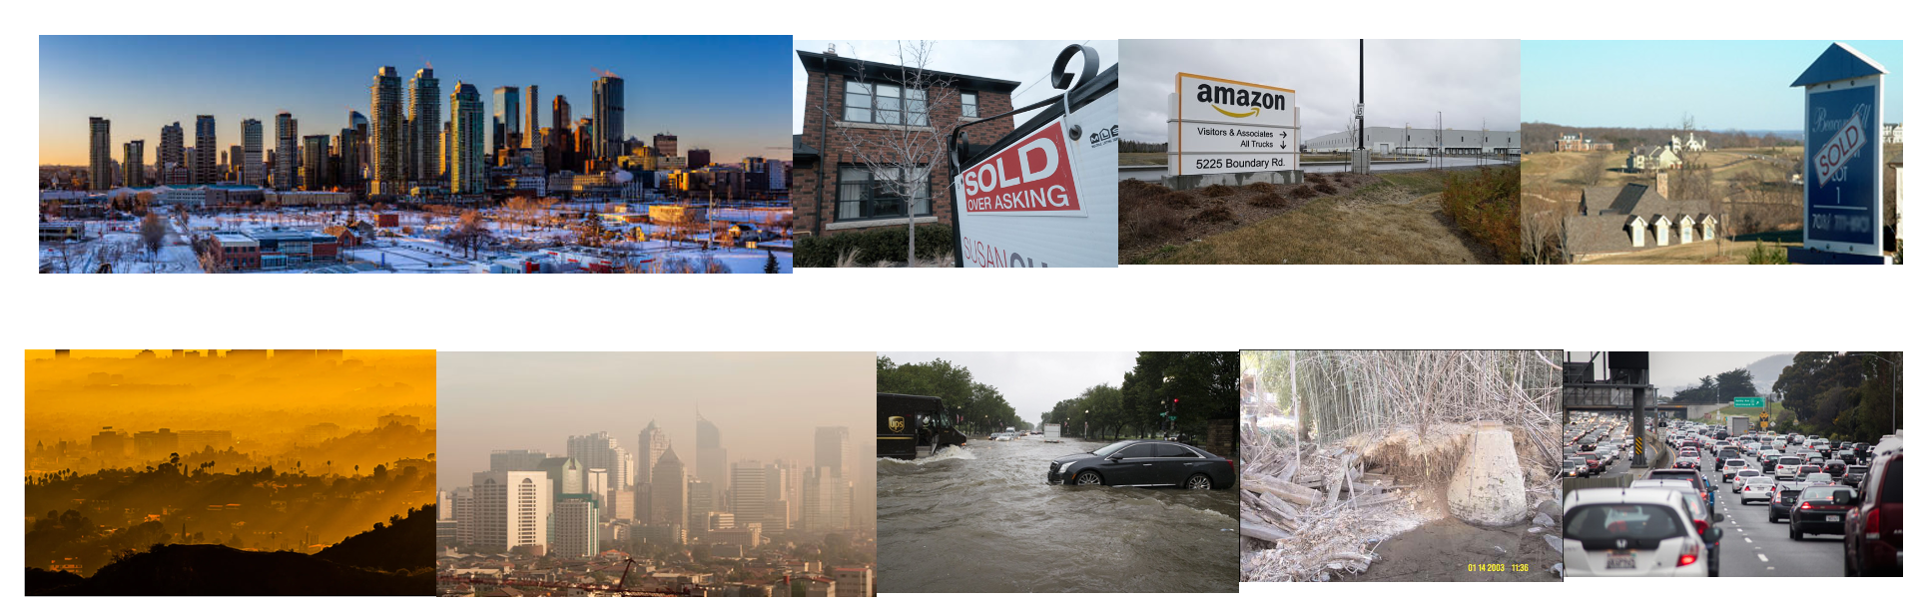
\includegraphics[scale=.15]{fig/example_figures/pictures-ex-1.png}
\end{frame}
\begin{frame}{Frame Title}
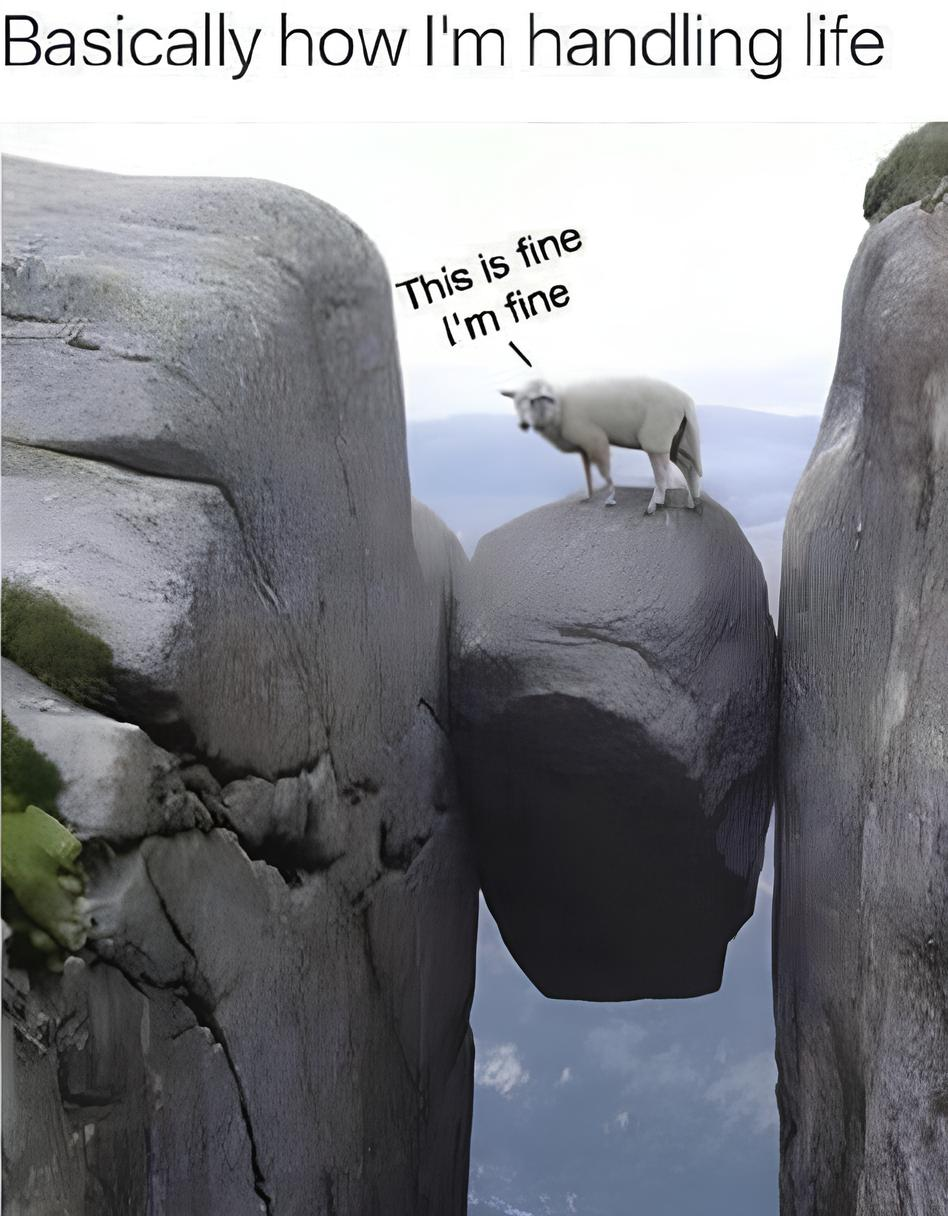
\includegraphics[scale=.25]{fig/sheep.jpg}
\end{frame}



% %----------------------------%
% %----------------------------%
% %----------------------------%
% %----------------------------%
% %----------------------------%
% %----------------------------%
% %----------------------------%
% %----------------------------%
% %----------------------------%
% %----------------------------%
% %----------------------------%
% %----------------------------%
% %----------------------------%
% %----------------------------%
% %----------------------------%
% %----------------------------%
% %----------------------------%
% %----------------------------%
% %----------------------------%
% %----------------------------%
% %----------------------------%
% %----------------------------%
% %----------------------------%
% %----------------------------%
% %----------------------------%
% %----------------------------%
% %----------------------------%
% %----------------------------%
% %----------------------------%
% %----------------------------%
% %----------------------------%
% %----------------------------%
% %----------------------------%
% %----------------------------%
% %----------------------------%
% %----------------------------%
% %----------------------------%
% %----------------------------%
% %----------------------------%
% %----------------------------%
% %----------------------------%
% %----------------------------%
% %----------------------------%
% %----------------------------%
% %----------------------------%


%% Example content %%
%%%%%%%%%%%%%%%%%%%%%%%%%%%%%%%%
%%%%%%%%%%%%%%%%%%%%%%%%%%%%%%%%

% %----------------------------%
% % Contents slide
% \begin{frame}
% \frametitle{Outline}
% \tableofcontents
% \end{frame}
% %----------------------------%

% %now include the slides
% \setbeamercovered{transparent}
% %----------------------------%
% \section{Section 1}
% \subsection{Subsection a}

% \begin{frame}
%     \frametitle{First slide Title}
%     \small
%     Add your contents and citations %\citep{Tantau2016beamerguide}
% \end{frame}
% \section{Section 2}
% \begin{frame}
%     \frametitle{Another Slide}
%     \small
%     Maybe some figures like Fig.~\ref{fig:my_label}
%     \begin{figure}
%         \centering
%         \includegraphics[width=3cm]{example-image-a}
%         \caption{Example image}
%         \label{fig:my_label}
%     \end{figure}
% \end{frame}
% %----------------------------%

% %----------------------------%
% % Conclusions
% \begin{frame}
%     \frametitle{}
%     \centering
    
%     \Large\color{titlecolor}
%     Thank you!

%     \vspace{0.5cm}
%     kirsten.wright@uwaterloo.ca

% \end{frame}
% %----------------------------%

% % References slide
% \begin{frame}
% \frametitle{References}
% \small
% % \bibliographystyle{apalike} %use the apalike bibliography style
% \bibliography{thesis-bib} % bibliography file
% \end{frame}

\end{document}
%%%%%%%%%%%%%%%%%%%%%%%%%%%%%%%%
%%%%%%%%%%%%%%%%%%%%%%%%%%%%%%%%